% ----------------------------------------------------
% Literature Review
% ----------------------------------------------------
\documentclass[class=report,11pt,crop=false]{standalone}
% Page geometry
\usepackage[a4paper,margin=25mm,top=25mm,bottom=25mm]{geometry}

% Font choice
\usepackage{lmodern}

% Use IEEE bibliography style
\bibliographystyle{IEEEtran}

% Line spacing
\usepackage{setspace}
\setstretch{1.20}

% Ensure UTF8 encoding
\usepackage[utf8]{inputenc}

% Language standard (not too important)
\usepackage[english]{babel}

% Skip a line in between paragraphs
\usepackage{parskip}

% For the creation of dummy text
\usepackage{blindtext}

% Math
\usepackage{amsmath}

% Header & Footer stuff
\usepackage{fancyhdr}
\pagestyle{fancy}
\fancyhead{}
\fancyhead[R]{\nouppercase{\rightmark}}
\fancyfoot{}
\fancyfoot[C]{\thepage}
\renewcommand{\headrulewidth}{0.0pt}
\renewcommand{\footrulewidth}{0.0pt}
\setlength{\headheight}{13.6pt}

% Page geometry
\usepackage[a4paper,top=25mm,bottom=25mm]{geometry}

% Epigraphs
\usepackage{epigraph}
\setlength\epigraphrule{0pt}

% Hyperlinks & References
\usepackage{hyperref}
\hypersetup{
    colorlinks=true,
    linkcolor=blue,
    filecolor=blue,      
    urlcolor=blue,
    citecolor=blue,
}
\urlstyle{same}

% Automatically correct front-side quotes
\usepackage[autostyle=false, style=american]{csquotes}
\MakeOuterQuote{"}

% Graphics
\usepackage{graphicx}
\graphicspath{{Images/}{../Images/}}

% Colour
\usepackage{color}
\usepackage[usenames,dvipsnames]{xcolor}

% SI units
\usepackage{siunitx}

% Microtype goodness
\usepackage{microtype}

% Listings
\usepackage{listings}
\definecolor{backgroundColour}{RGB}{250,250,250}
\definecolor{commentColour}{RGB}{73, 175, 102}
\definecolor{identifierColour}{RGB}{196, 19, 66}
\definecolor{stringColour}{RGB}{252, 156, 30}
\definecolor{keywordColour}{RGB}{50, 38, 224}
\definecolor{lineNumbersColour}{RGB}{127,127,127}
\lstset{ 
  language=Matlab,
  captionpos=b,
  backgroundcolor=\color{backgroundColour},
  basicstyle=\footnotesize,        % the size of the fonts that are used for the code
  breakatwhitespace=false,         % sets if automatic breaks should only happen at whitespace
  breaklines=true,                 % sets automatic line breaking
  postbreak=\mbox{\textcolor{red}{$\hookrightarrow$}\space},
  commentstyle=\color{commentColour},    % comment style
  identifierstyle=\color{identifierColour},
  stringstyle=\color{stringColour},
   keywordstyle=\color{keywordColour},       % keyword style
  %escapeinside={\%*}{*)},          % if you want to add LaTeX within your code
  extendedchars=true,              % lets you use non-ASCII characters; for 8-bits encodings only, does not work with UTF-8
  frame=single,	                   % adds a frame around the code
  keepspaces=true,                 % keeps spaces in text, useful for keeping indentation of code (possibly needs columns=flexible)
  morekeywords={*,...},            % if you want to add more keywords to the set
  numbers=left,                    % where to put the line-numbers; possible values are (none, left, right)
  numbersep=5pt,                   % how far the line-numbers are from the code
  numberstyle=\tiny\color{lineNumbersColour}, % the style that is used for the line-numbers
  rulecolor=\color{black},         % if not set, the frame-color may be changed on line-breaks within not-black text (e.g. comments (green here))
  showspaces=false,                % show spaces everywhere adding particular underscores; it overrides 'showstringspaces'
  showstringspaces=false,          % underline spaces within strings only
  showtabs=false,                  % show tabs within strings adding particular underscores
  stepnumber=1,                    % the step between two line-numbers. If it's 1, each line will be numbered
  tabsize=2,	                   % sets default tabsize to 2 spaces
  %title=\lstname                   % show the filename of files included with \lstinputlisting; also try caption instead of title
}

% Caption stuff
\usepackage{caption}
\usepackage{subcaption}

% \makenoidxglossaries

\newacronym{radar}{RADAR}{Radio Detection and Ranging}
\newacronym{dab}{DAB}{Digital Audio Broadcasting}
\newacronym{fm}{FM}{Frequency Modulation}
\newacronym{am}{AM}{Amplitude Modulation}
\newacronym{fdm}{FDM}{Frequency Division Multiplexing}
\newacronym{ofdm}{OFDM}{Orthogonal Frequency Division Multiplexing}
\newacronym{cofdm}{COFDM}{Coded Orthogonal Frequency Division Multiplexing}
\newacronym{dvbt2}{DVB–T2}{Digital Video Broadcasting — Second Generation Terrestrial}
\newacronym{em}{EM}{electromagnetic}
\newacronym{icasa}{ICASA}{Independent Communications Authority of South Africa}
\newacronym{ioo}{IOO}{Illuminators of Opportunity}
\newacronym{pr}{PR}{Passive Radar}
\newacronym{qpsk}{QPSK}{Differential Quadrature Phase-Shift Keying}
\newacronym{dqpsk}{DQPSK}{Differential Quadrature Phase-Shift Keying}
\newacronym{etsi}{ETSI}{European Telecommunications Standards Institute}
\newacronym{psk}{PSK}{Phase Shift Keying}
\newacronym{ask}{ASK}{Amplitude-Shift Keying}
\newacronym{fsk}{FSK}{Frequency-Shift Keying}
\newacronym{iq}{IQ}{In-phase and Quadrature}
\newacronym{prs}{PRS}{Phase Reference Symbol}
\newacronym{dft}{DFT}{Discrete Fourier Transform}
\newacronym{fft}{FFT}{Fast Fourier Transform}
\begin{document}
% ----------------------------------------------------
\chapter{Proofs}
% ----------------------------------------------------

\section{Effect of Windowing in the Frequency Domain}

Any physically-realizable system can only ever consider a finite section of a received signal---over the integration period. Mathematically, this is equivalent to multiplying the signal by a windowing function, \(w(t)\).

To understand why, consider a carrier wave, \(f(t)\), which has a frequency of \(\omega_0\) and is recorded over a period of \(T\) seconds. Notice that this is equivalent to multiplying \(f(t)\) by a windowing function, \(w(t)\), with a width of \(T\). Figure~\ref{fig:sampling-sine} depicts this, where a simple rectangular pulse is used as the windowing function. Note, however, that more complex windowing functions can be used, and the point will remain. The resulting windowed carrier wave is notated as \(f_T(t)\).

\begin{figure}[htbp]
    \centering
    \captionsetup{type=figure}
    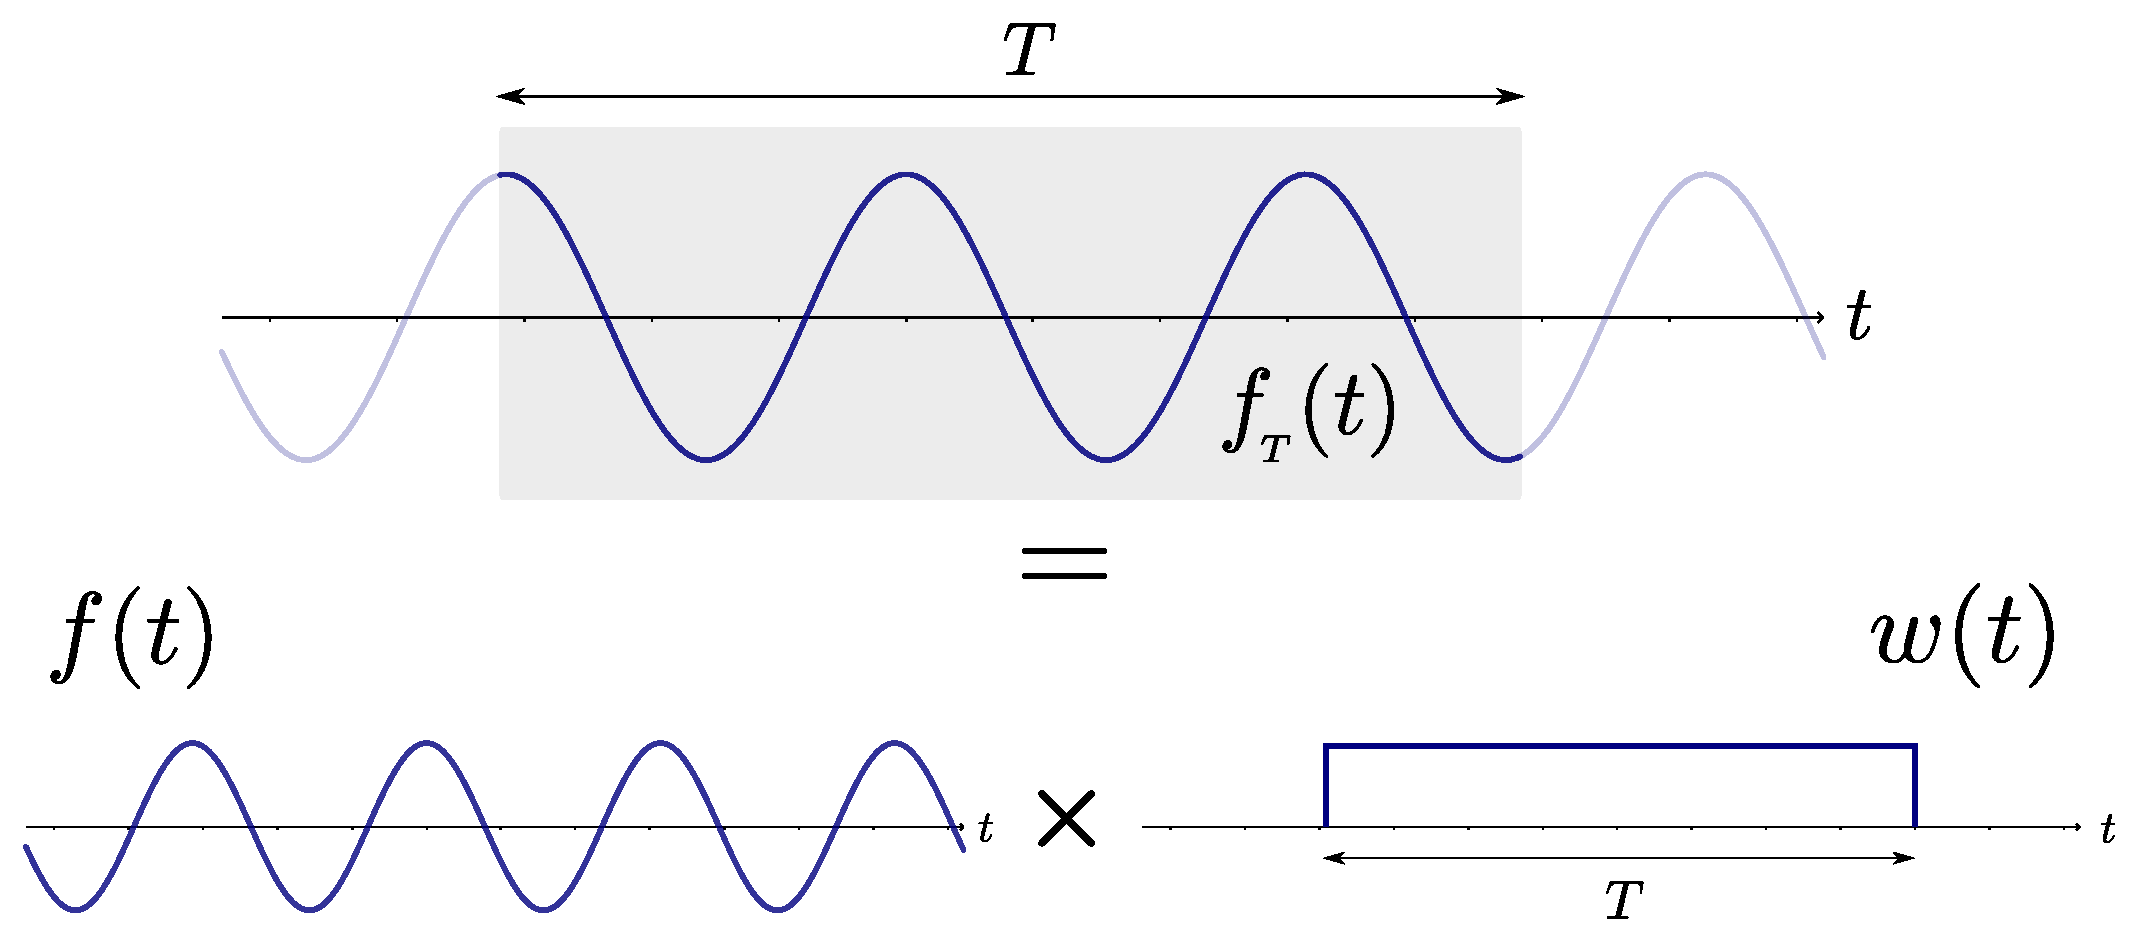
\includegraphics[width=0.7\linewidth]{sampling-sine.pdf}
    \caption{Depiction of sampling as a multiplication with a finite window function}
    \label{fig:sampling-sine}
\end{figure}

Consider now the impact of windowing as viewed in the frequency domain. The original carrier wave, \(f(t)\), which theoretically spans over all time, is perfectly impulsive. However, multiplication with the windowing function in time is equivalent to convolution with the window's spectrum in frequency. The exact details of this spectrum depend on the windowing function used, but for a simple rectangular function,
\begin{equation}
    w(t) = \textrm{rect}\bigg(\frac{t}{T}\bigg) \xLeftrightarrow{\quad\mathcal{F}\quad} W(\omega) = T \cdot \textrm{Sa}\bigg(\frac{\omega T}{2}\bigg)
\end{equation}
where \(\textrm{Sa}(x)=\frac{\sin{x}}{x}\).

\begin{figure}[htbp]
    \centering
    \captionsetup{type=figure}
    \def\svgwidth{\linewidth}
    {\setstretch{0.7} % Line spacing
        \input{../Images/sampling-sine-freq.pdf_tex}}
    \caption{Effect of windowing on spectrum}
    \label{fig:sampling-sine-freq}
\end{figure}

\section{OFDM Carrier Orthogonality: Time Domain \label{sect:proofs_ofdm-time}}

% \begin{lemma}
    Given two complex exponential signals with frequencies that differ by \(\frac{k}{T}\), the signals are orthogonal over an integration period of~\(T\) for any integer value of~\(k\).

\begin{proof}
    Consider two complex exponential signals,
    
    \begin{equation}
        \psi_1 = \rho_1 \cdot e^{j(2\pi f_0 t + \theta_1)}
    \end{equation}
    \begin{equation}
        \psi_2 = \rho_2 \cdot e^{j(2\pi (f_0 + \frac{k}{T})t + \theta_2)}
    \end{equation}

    Looking at the orthogonality of the signals:
    
    % \begin{equation}
        \setlength{\jot}{10pt}
        \begin{align}
            F &= \int_0^T \psi_1(t) \psi_2^*(t) dt \\
            &= \int_0^T \rho_1 e^{j(2\pi f_0 t + \theta_1)} \cdot \rho_2 e^{-j(2\pi (f_0 + \frac{k}{T})t + \theta_2)} dt \\
            &= \rho_1 \rho_2 \int_0^T e^{j(2\pi f_0 t + \theta_1 - 2\pi f_0 t - 2\pi \frac{k}{T}t - \theta_2)} dt \\
            &= \rho_1 \rho_2 e^{j(\theta_1 - \theta_2)} \int_0^T e^{-j 2\pi \frac{k}{T} t} dt \\
            &= \rho_1 \rho_2 e^{j(\theta_1 - \theta_2)} \cdot \frac{1}{-j2\pi\frac{k}{T}} \bigg[ e^{-j2\pi\frac{k}{T} t} \bigg]^{t=T}_{t=0} \\
            &= \rho_1 \rho_2 e^{j(\theta_1 - \theta_2)} \cdot \frac{1}{-j2\pi\frac{k}{T}} (e^{-j2\pi k} - 1) \\
            &= \rho_1 \rho_2 e^{j(\theta_1 - \theta_2)} \cdot \frac{1}{-j2\pi\frac{k}{T}} \cdot 0 = 0
        \end{align}
    % \end{equation}
    
\end{proof}


\section{OFDM Carrier Orthogonality: Frequency Domain \label{sect:proofs_ofdm-freq}}

\section{Using the DFT in OFDM systems}


% ----------------------------------------------------
\ifstandalone
% \bibliography{../Bibliography/References.bib}
% \printnoidxglossary[type=\acronymtype,nonumberlist]
\fi
\end{document}
% ----------------------------------------------------